232. \begin{figure}[ht!]
\center{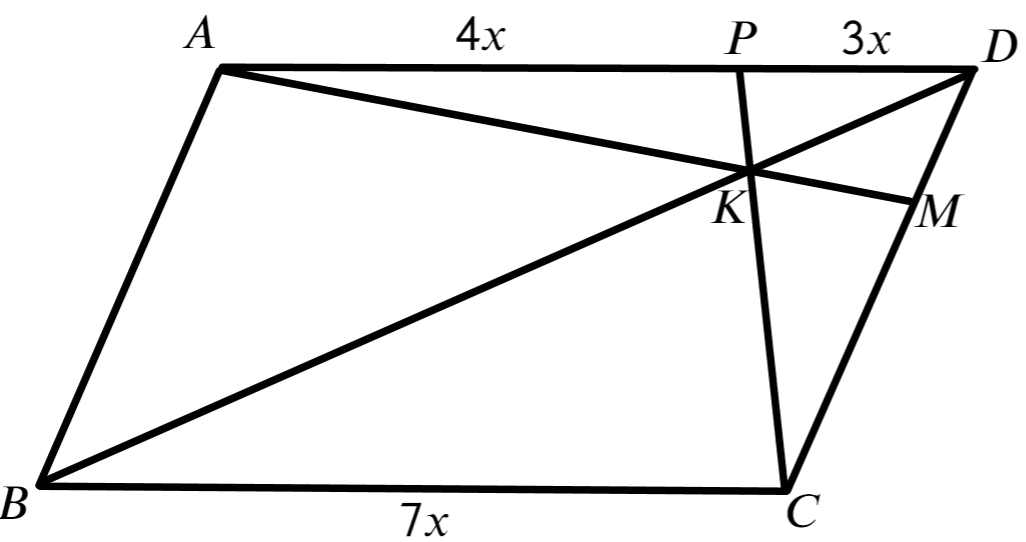
\includegraphics[scale=0.35]{g8-232.png}}
\end{figure}\\
Пусть $AP=4x,$ а $PD=3x,$ тогда $BC=AD=4x+3x=7x.$ Треугольники $DPK$ и $BCK$ подобны по двум углам ($\angle PDK=\angle KBC$ и $\angle DPK=\angle BCK$ как накрест лежащие), поэтому $\cfrac{BK}{KD}=\cfrac{BC}{PD}=\cfrac{7x}{3x}=\cfrac{7}{3}.$ Треугольники $ABK$ и $DKM$ аналогично подобны по двум углам, значит $\cfrac{AB}{DM}=\cfrac{BK}{KD}=\cfrac{7}{3}.$ Тогда $\cfrac{CD}{DM}=\cfrac{AB}{DM}=\cfrac{7}{3},$ значит $DM=\cfrac{3}{7}CD,\ CM=CD-DM=\cfrac{4}{7}CD,\ CM:MD=\cfrac{4}{7}:\cfrac{3}{7}=4:3.$\\
